\section{Introduction}
Building distributed frameworks to facilitate model training on large and growing datasets is a key data management challenge with significant interest in both industry and academia~\cite{bdas, alexandrov2014stratosphere, crotty2014tupleware, tensor}.
While these frameworks abstract much of the difficult details of distributed Machine Learning (ML), they seldom offer the analyst any support in terms of constructing the model itself, such as which features to use or how to represent their data.
The model construction process is still highly iterative, where through trial-and-error an analyst makes these choices eventually converging onto a model with the desired accuracy.
To further complicate matters, data often arrives \emph{dirty}, including missing, incorrect, or inconsistent attributes, due to faulty sensors, software, time delays, or hardware.
Thus, part of the iterative model construction process involves identifying potentially dirty data, understanding how they affect the model, and applying techniques to mitigate their effects.  
While data cleaning is an extensively studied problem, the high dimensionality of many models can amplify even a small amount of erroneous records~\cite{xiaofeature}, and the relative complexity (in comparison to SQL analytics) can make it difficult to trace the consequnces of an error.

\begin{figure}[t]
\centering
 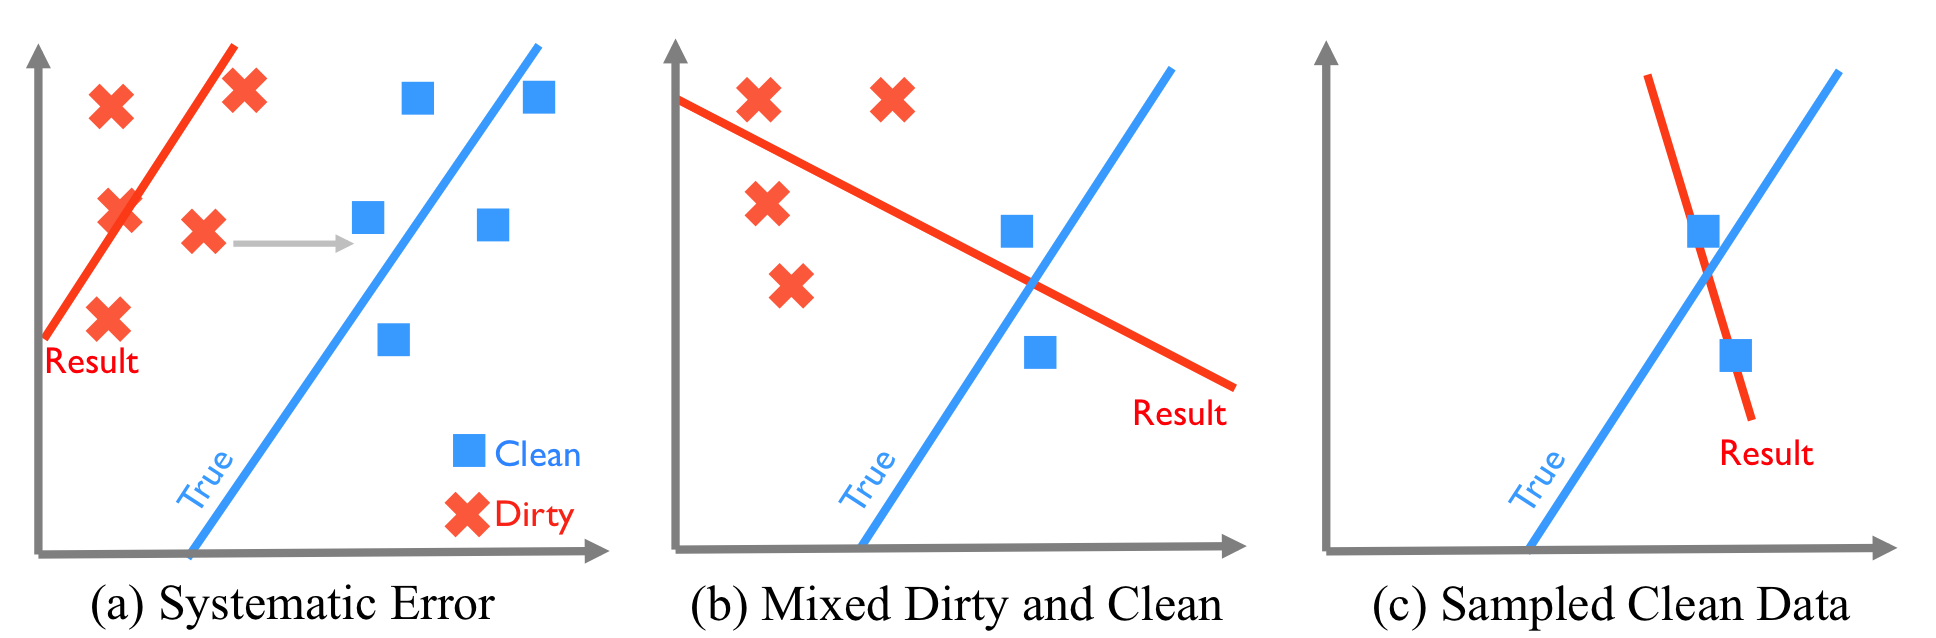
\includegraphics[width=\columnwidth]{figs/update-arch.png}
 \caption{(a) Systematic corruption in one variable can lead to a shifted model. 
 (b) Mixed dirty and clean data results in a less accurate model than no cleaning.
(c) Small samples of only clean data can result in similarly inaccurate models. \label{update-arch1}}
\end{figure}

In prior work, we have noted the choice of data cleaning algorithm can significantly affect results even when using robust ML techniques \cite{activecleanarxiv, DBLP:conf/case/MahlerKLSMKPWFAG14}.
In one fraud prediction example, we found that simply applying Entity Resolution before model training improved true positive detection probabilities from 62\% to 91\%. 
Despite this importance, in theory and in practice, the academic community has decoupled the data cleaning problem from featurization and ML.
This is problematic because many ML techniques often make assumptions about data homogeneity and the consistency of sampling, which can be easily violated if the analyst applies data cleaning in an arbitrary way.

To understand how this may happen, consider an anlyst training a regression model on dirty data. At first, she may not realize that there are outliers and train an initial model directly on the dirty data. 
As she starts to inspect the model, she may realize that some records have a large residual value (not predicted accurately). 
Once she confirms that those records are indeed dirty, she has to design data cleaning rules or scripts to fix or remove the offending records. 
After cleaning, she re-trains the model--iterating until she no longer finds dirty data.
This iterative process is the de facto standard, and in fact encouraged by the design of the increasingly popular interactive ``notebook" ML development environments (e.g., IPython), but makes the implicit assumption that model training commutes with incremental data cleaning.
This assumption is wholly incorrect; due to the well-known Simpson's paradox, models trained on a mix of dirty and clean data can have very misleading results even in simple scenarios (Figure \ref{update-arch1}).

In a parallel trend, the dimensionality of the features used in ML models is also rapidly increasing. 
It is now common to use 100,000s of features in image processing processing problems with techniques such as Deep Learning.
Empirically, such feature spaces have facilitated breakthroughs in previously hard classification tasks such as image classification, robot actuation, and speech recognition.
However, the pitfall is that the standard approaches for debugging and reasoning about data error may lose their intuition for higher dimensions.
In other words, it is often not obvious how an analyst should select which records to clean.

As it stands, there are two key problems in interactive model construction, (1) correctness, and (2) dirty data identification.
We address these to problems in a system called \sys which facilitates interactive training-cleaning iteration in a safe way (with expected monotone convergence guarantees) and automatically selects the most valuable data for the analyst to inspect even in the complex models popular in modern ML pipelines.
The selection technique applied in \sys uses pointwise gradients to generalize the outlier filtering heuristics to select potentially dirty data even in complex models. 
The analyst initializes an \sys with an ML model, a featurization function, and the base data, and the \sys initially returns the model trained on the dataset.
\sys also returns an array of data sampled from the model that are possibly dirty.
The analyst can apply any value transformations to the data and then prompt the system to iterate. 

We demonstrate \sys with a visual interface allows analysts to debug complex ML models and understand the effects of dirty data.
This interface will allow the analyst to specify the desired model and featurization.
It will then visualize a sample of potentially dirty records and allow the analyst to clean the data appropriately.  
In our demonstration, we will present three experimental scenarios where the models are affected by dirty data: 

\begin{example}[Event Detection With SVMs]


\end{example}

\begin{example}[Video Segmentation With CNNs]

\end{example}

\begin{example}[Topic Modeling With LDA]

\end{example}
 









